% Chapter 3: System Architecture and Methodology

\chapter{System Architecture and Methodology}
\label{chap:methods}

\section{System Overview: The 12-Module Gateway}
The proposed serving system is organized into twelve modular subsystems (\textbf{M1} through \textbf{M12}) operating as an asynchronous, OpenAI-compatible proxy gateway. Figure \ref{fig:risk_curve} illustrates the empirical risk trajectory and threshold calibration governing this architecture.

\begin{figure}[htbp]
    \centering
    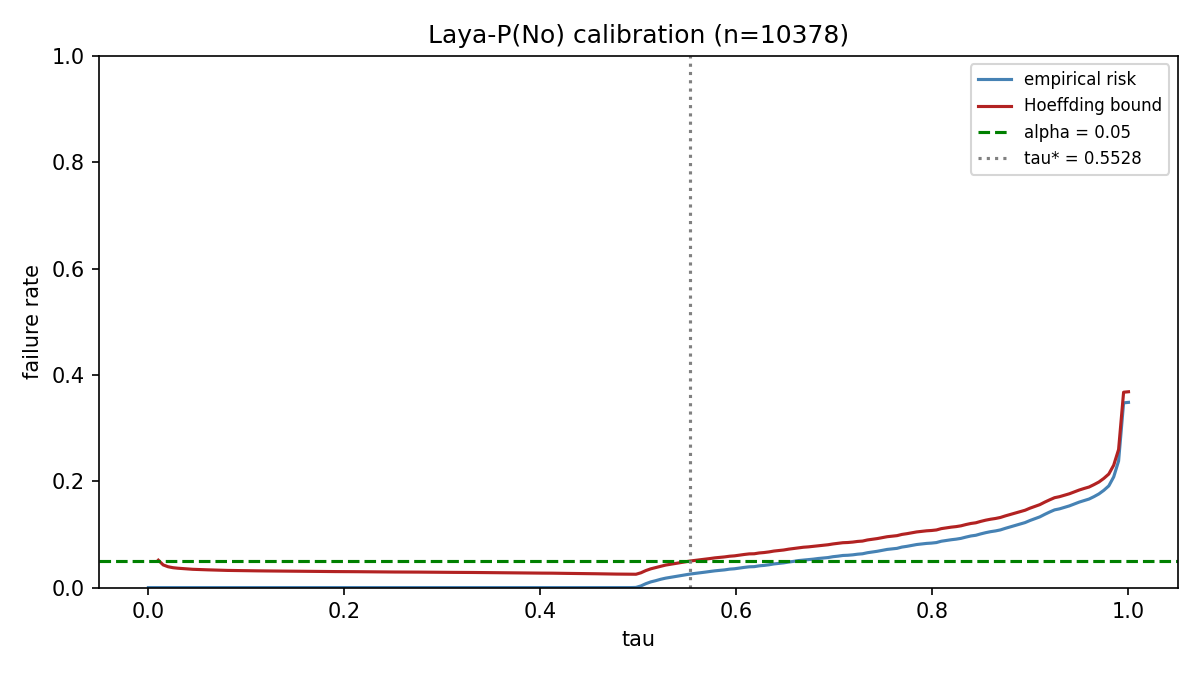
\includegraphics[width=0.85\linewidth]{Figures/fig_risk_laya.png}
    \caption{Empirical risk curve and Hoeffding upper confidence bounds evaluated over the ModernBERT router across candidate thresholds $\tau$.}
    \label{fig:risk_curve}
\end{figure}

The functional taxonomy of the 12 gateway modules is formalized in Table \ref{tab:gateway_modules}.

\begin{table}[htbp]
\centering
\small
\caption{Taxonomy of the 12 Modules in the Code-Mixed Serving Gateway.}
\label{tab:gateway_modules}
\begin{tabularx}{\textwidth}{lp{4.2cm}X}
\toprule
\textbf{Module} & \textbf{Designation} & \textbf{Core Functionality} \\
\midrule
\textbf{M1} & \texttt{m1\_pipeline} & Tokenization benchmarking (tiktoken, MuRIL) and \texttt{code\_mix\_ratio()} estimation. \\
\textbf{M2} & \texttt{m2\_compressor} & 5-stage CPU compressor: phonetic hashing, regex protection, and Linear-Chain CRF tagger. \\
\textbf{M3} & \texttt{m3\_conformal} & Conformal risk control: Hoeffding/LTT threshold selection and Clopper-Pearson UCB. \\
\textbf{M4} & \texttt{m4\_router} & Cascade router: ModernBERT $P(\text{No})$ difficulty scoring and model dispatch. \\
\textbf{M5} & \texttt{m5\_gateway} & Central FastAPI serving engine supporting 20+ endpoints, SSE streaming, and receipts. \\
\textbf{M6} & \texttt{m6\_telegram} & Telegram bot interface with SQLite audit logging for live mobile user testing. \\
\textbf{M7} & \texttt{m7\_eval} & Evaluation suite computing BLEU, ROUGE-L, and exact-match task success. \\
\textbf{M8} & \texttt{m8\_dashboard} & Telemetry aggregator providing real-time savings and routing statistics. \\
\textbf{M9} & \texttt{m9\_reasoning} & Reasoning budget estimator quantifying internal thinking token disparities. \\
\textbf{M10} & \texttt{m10\_train} & Training and distillation scaffolding for reward models and GRPO configs. \\
\textbf{M11} & \texttt{m11\_calibration} & Uncertainty calibration via Expected Calibration Error (ECE) and reliability diagrams. \\
\textbf{M12} & \texttt{m12\_novel} & Adaptive compression budgeting ($0.52 + 0.30\cdot\text{mix} + 0.18\cdot\text{diff}$) and semantic glossing. \\
\bottomrule
\end{tabularx}
\end{table}

\section{Pipeline Pre-Processing: Tokenizer Analysis (M1)}
Module M1 inspects every incoming query $x$ prior to compression. It computes the code-mixing ratio $\mu(x) \in [0, 1]$:
\begin{equation}
    \mu(x) = \frac{N_{\text{Devanagari}}(x) + N_{\text{Romanized}}(x)}{N_{\text{Total}}(x)}
\end{equation}
where $N_{\text{Devanagari}}(x)$ denotes tokens matching unicode range \texttt{[\textbackslash u0900-\textbackslash u097f]}, and $N_{\text{Romanized}}(x)$ denotes tokens matching a curated lexicon of 100+ high-frequency Hindi function words, pronouns, and verbs.

\section{The 5-Stage CPU Prompt Compressor (M2)}
Prompt compression in M2 operates entirely on CPU without GPU overhead ($<10$\,ms per turn), adhering to five sequential stages:

\subsection{Stage 1: Phonetic Consonant-Skeleton Hashing}
Romanized Hindi exhibits severe spelling entropy. To collapse morphological variance into stable representations, we introduce the \texttt{hinglish\_phash} algorithm. For each token:
\begin{enumerate}
    \item Convert to lowercase and expand known colloquial abbreviations (e.g., \textit{``kr''} $\to$ \textit{``kar''}).
    \item Collapse character runs of 3+ identical characters to a single character (e.g., \textit{``heyyyy''} $\to$ \textit{``hey''}).
    \item Map aspirated consonant clusters to invariant single tokens: \texttt{sh}$\to$\texttt{S}, \texttt{ch}$\to$\texttt{C}, \texttt{th}$\to$\texttt{T}, \texttt{dh}$\to$\texttt{D}, \texttt{kh}$\to$\texttt{K}, \texttt{gh}$\to$\texttt{G}, \texttt{ph}$\to$\texttt{F}, \texttt{bh}$\to$\texttt{B}.
    \item Strip vowels and trailing inflectional suffixes, producing a canonical consonant skeleton (e.g., \textit{raha}, \textit{rha}, \textit{rahi} all map to \texttt{RH*}).
\end{enumerate}

\subsection{Stage 2: Deterministic Heuristic Pre-Pruning}
Before invoking machine learning classifiers, context-free deterministic passes prune conversational greetings (\textit{``good morning''}, \textit{``namaste''}), collapse adjacent and echo reduplications (\textit{``jaldi jaldi''} $\to$ \textit{``jaldi''}; \textit{``chai-vai''} $\to$ \textit{``chai''}), and strip 8 unambiguous conversational fillers (\textit{arre, arey, um, uh, umm, err, hmm}).

\subsection{Stage 3: Protected-Span Safety Masking}
To prevent entity destruction, a deterministic regular expression pass detects critical structured information:
\begin{equation}
    \mathcal{S} = \{ \text{emails, URLs, phone numbers, timestamps, monetary amounts, code blocks} \}
\end{equation}
Each detected span $s_k \in \mathcal{S}$ is extracted, stored in memory, and replaced in the text by a synthetic invariant token \texttt{[[PSk]]} (or \texttt{ZXPROTECTED\_k}). The downstream token classifier is explicitly forced to retain all \texttt{[[PSk]]} tokens.

\subsection{Stage 4: Linear-Chain CRF Sequence Tagger}
We formulate token retention as sequence labeling using a Linear-Chain Conditional Random Field (CRF) \cite{lafferty2001conditional}. Given input token sequence $\mathbf{x} = (x_1, \dots, x_n)$, the model predicts binary labels $\mathbf{y} = (y_1, \dots, y_n) \in \{0, 1\}^n$:
\begin{equation}
    p(\mathbf{y} \mid \mathbf{x}) = \frac{1}{Z(\mathbf{x})} \exp \left( \sum_{i=1}^n \sum_{k} \lambda_k f_k(y_{i-1}, y_i, \mathbf{x}, i) \right)
\end{equation}
Each token is characterized by 25+ linguistic features:
\begin{itemize}
    \item \textbf{Orthographic:} Lowercase form, phonetic hash, prefix/suffix lengths 1--3, character length.
    \item \textbf{Syntactic \& Informational:} TF-IDF weight, frequency decile, boolean punctuation/digit flags.
    \item \textbf{Positional:} Relative position ratio ($i/n$), first/last token flags.
    \item \textbf{Contextual Window:} $\pm 2$ neighbor tokens with their respective phonetic hashes and suffixes.
\end{itemize}
Viterbi decoding yields the optimal global retention sequence $\mathbf{y}^*$ in linear time $\mathcal{O}(n)$.

\subsection{Stage 5: Fail-Closed Post-Compression Reinjection}
Surviving tokens are reassembled according to their original sentence indices. A verification pass matches all original \texttt{[[PSk]]} placeholders:
\begin{equation}
    \text{Reinject}(\mathbf{x}_{\text{comp}}, \mathcal{S}) = 
    \begin{cases}
        \text{Replace } \texttt{[[PSk]]} \to s_k, & \text{if all } s_k \text{ accounted for} \\
        \mathbf{x}_{\text{original}}, & \text{if any } \texttt{[[PSk]]} \text{ dropped (Fail-Closed)}
    \end{cases}
\end{equation}
This mathematical guarantee ensures that entity corruption is completely impossible in production.

\section{Conformal Cascade Routing (M4 \& M3)}
Queries exiting compression are evaluated by the Cascade Router to choose between a compact model (Groq Llama-3-8B) and a frontier model (GPT-4o).

\subsection{Difficulty Scoring with ModernBERT-large}
We fine-tune ModernBERT-large (395M parameters) \cite{modernbert2024} to estimate the probability that the cheap model will fail on prompt $x$:
\begin{equation}
    d(x) = \mathbb{P}(\text{Cheap Model Fails} \mid x) = P(\text{No} \mid x) \in [0, 1]
\end{equation}

\begin{figure}[htbp]
    \centering
    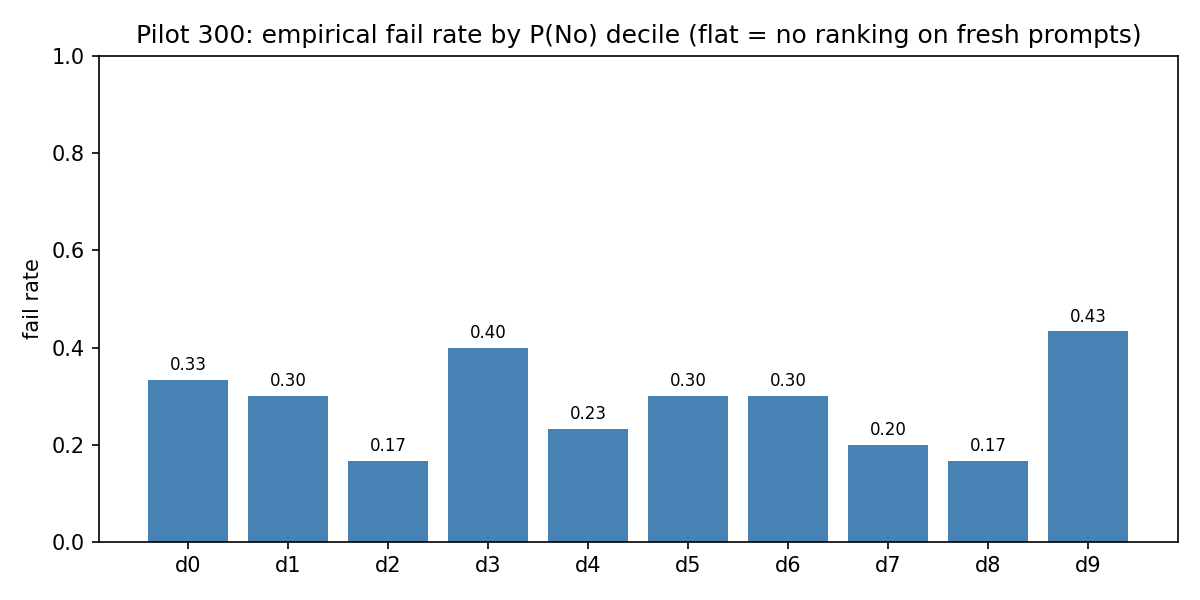
\includegraphics[width=0.85\linewidth]{Figures/fig_deciles.png}
    \caption{Decile calibration showing empirical cheap model failure rates monotonically aligned with router difficulty scores.}
    \label{fig:decile_calibration}
\end{figure}

\subsection{Risk-Controlled Threshold Selection}
Given a pre-specified failure budget $\alpha \in (0, 1)$ (e.g., $\alpha = 0.05$) and confidence $\delta = 0.05$, M3 calibrates threshold $\tau^*$ over a held-out calibration split $\mathcal{D}_{\text{cal}} = \{(x_j, y_j)\}_{j=1}^m$:
\begin{equation}
    \widehat{R}(\tau) = \frac{1}{m} \sum_{j=1}^m \mathbb{I}\Big( d(x_j) \le \tau \Big) \cdot \mathbb{I}\Big( \text{Cheap Model Failed on } x_j \Big)
\end{equation}
Using the Hoeffding Learn-Then-Test bound \cite{angelopoulos2024conformal}:
\begin{equation}
    R^+(\tau) = \widehat{R}(\tau) + \sqrt{\frac{\ln(1/\delta)}{2m}}
\end{equation}
The optimal threshold $\tau^*$ is selected as:
\begin{equation}
    \tau^* = \max \left\{ \tau \in [0, 1] : R^+(\tau) \le \alpha \right\}
\end{equation}
At inference: if $d(x) \le \tau^*$, dispatch to cheap model; otherwise, escalate to premium model.

\section{Adaptive Compression Policy (M12)}
To prevent over-compression on nuanced dialogue, Module M12 implements a mixture-aware adaptive target:
\begin{equation}
    \text{Target Kept Ratio} = \text{clip}\Big( 0.52 + 0.30 \cdot \mu(x) + 0.18 \cdot d(x), \; 0.38, \; 0.92 \Big)
\end{equation}
Heavily code-mixed queries ($\mu(x) \to 1$) and mathematically challenging prompts ($d(x) \to 1$) automatically receive higher token budgets, safeguarding conversational continuity.
